\documentclass[12pt]{article}

% Packages
\usepackage[margin=1in]{geometry}
\usepackage{fancyhdr}
\usepackage{amsmath, amsthm, amssymb, physics, graphicx}

% Page Style
\fancypagestyle{plain}{
    \fancyhf{}
    \renewcommand{\headrulewidth}{0pt}
    \renewcommand{\footrulewidth}{0pt}
    \fancyfoot[R]{\thepage}
}
\pagestyle{plain}

% Problem Box
\setlength{\fboxsep}{4pt}
\newsavebox{\savefullbox}
\newenvironment{fullbox}{\begin{lrbox}{\savefullbox}\begin{minipage}{\dimexpr\textwidth-2\fboxsep\relax}}{\end{minipage}\end{lrbox}\begin{center}\framebox[\textwidth]{\usebox{\savefullbox}}\end{center}}
\newenvironment{pbox}[1][]{\begin{fullbox}\ifx#1\empty\else\paragraph{#1}\fi}{\end{fullbox}}

% Options
\renewcommand{\thesubsection}{\thesection(\alph{subsection})}
\allowdisplaybreaks
\addtolength{\jot}{4pt}
\theoremstyle{definition}

% Default Commands
\newtheorem{proposition}{Proposition}
\newtheorem{lemma}{Lemma}
\newcommand{\ds}{\displaystyle}
\newcommand{\isp}[1]{\quad\text{#1}\quad}
\newcommand{\N}{\mathbb{N}}
\newcommand{\Z}{\mathbb{Z}}
\newcommand{\Q}{\mathbb{Q}}
\newcommand{\R}{\mathbb{R}}
\newcommand{\C}{\mathbb{C}}
\newcommand{\eps}{\varepsilon}
\renewcommand{\phi}{\varphi}
\renewcommand{\emptyset}{\varnothing}
\newcommand{\pfrac}[2]{\left(\frac{#1}{#2}\right)}

% Extra Commands


% Document Info
\fancypagestyle{title}{
    \renewcommand{\headrulewidth}{0.4pt}
    \setlength{\headheight}{15pt}
    \fancyhead[R]{Harry Coleman}
    \fancyhead[L]{GEOG 191 Lab 6}
    \fancyhead[C]{February 26, 2021}
}

% Begin Document
\begin{document}
\thispagestyle{title}


\begin{pbox}
    Solve the problem as a linear program (no integer requirements). 
\end{pbox}

\begin{center}
    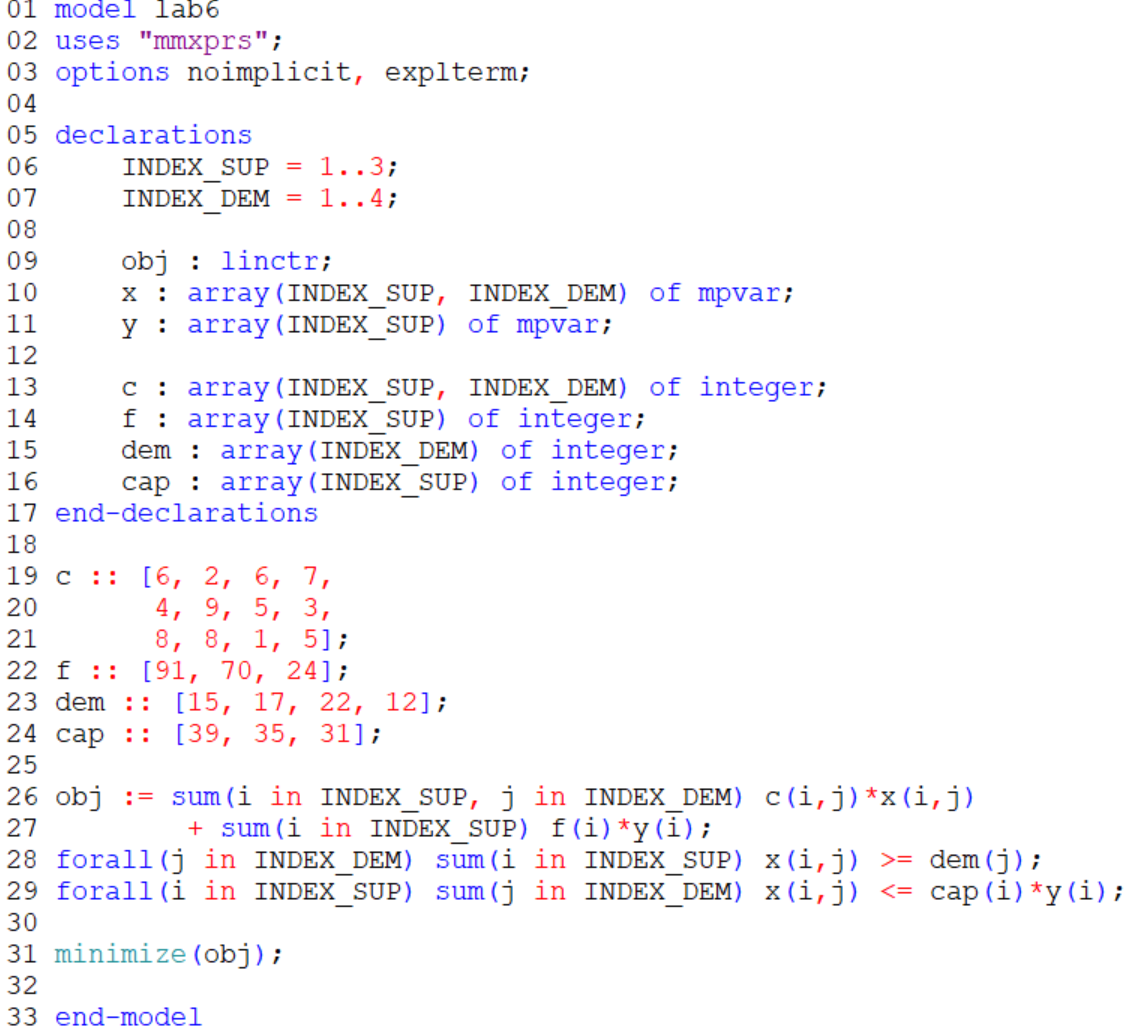
\includegraphics[width=\textwidth]{code1.png}
\end{center}



\newpage
\begin{pbox}
    Report the solution and solver details. Discuss whether the solution makes sense for planning and management decision making.
\end{pbox}

Running the above code, Xpress produces the following optimal solution using the simplex dual algorithm (7 iterations).
\[
    Z = 262.7
    \qquad
    x = \mqty[
        0 & 17 & 0 & 0 \\
        15 & 0 & 0 & 12 \\
        0 & 0 & 22 & 0
    ]
    \qquad
    y = \mqty[0.435897 \\ 0.771429 \\ 0.709677]
\]
The values of $y$ in this solution do not make sense in the original problem, as their purpose is to tell us whether or not a particular factory is to be upgraded and kept open. In the case that a factory is selected (e.g., if $y_i = 1$ then factory $i$ is selected), then an associated fixed cost, reflecting the cost of upgrades and future maintenance, is meant to be added to the objective (total cost), regardless of how many units it will produce. However, the above program uses the fractional $y$ values to scale the fixed costs for each factory by how much they produce proportional to their maximum capacity (meaning that the value of the objective function is also nonsensical). This behavior does not reflect the actual problem, nor can the solution it produced be directly interpreted as a solution to the actual problem.

If necessary, we could interpret it by rounding all $y$ values up to $1$ and using the production quantities given for each factory. The actual objective value would be higher than shown, but we would technically be able to implement the above solution in the original problem, though it is unlikely to be an optimal solution. 



\newpage
\begin{pbox}
    Solve the problem as an integer program.
\end{pbox}

\begin{center}
    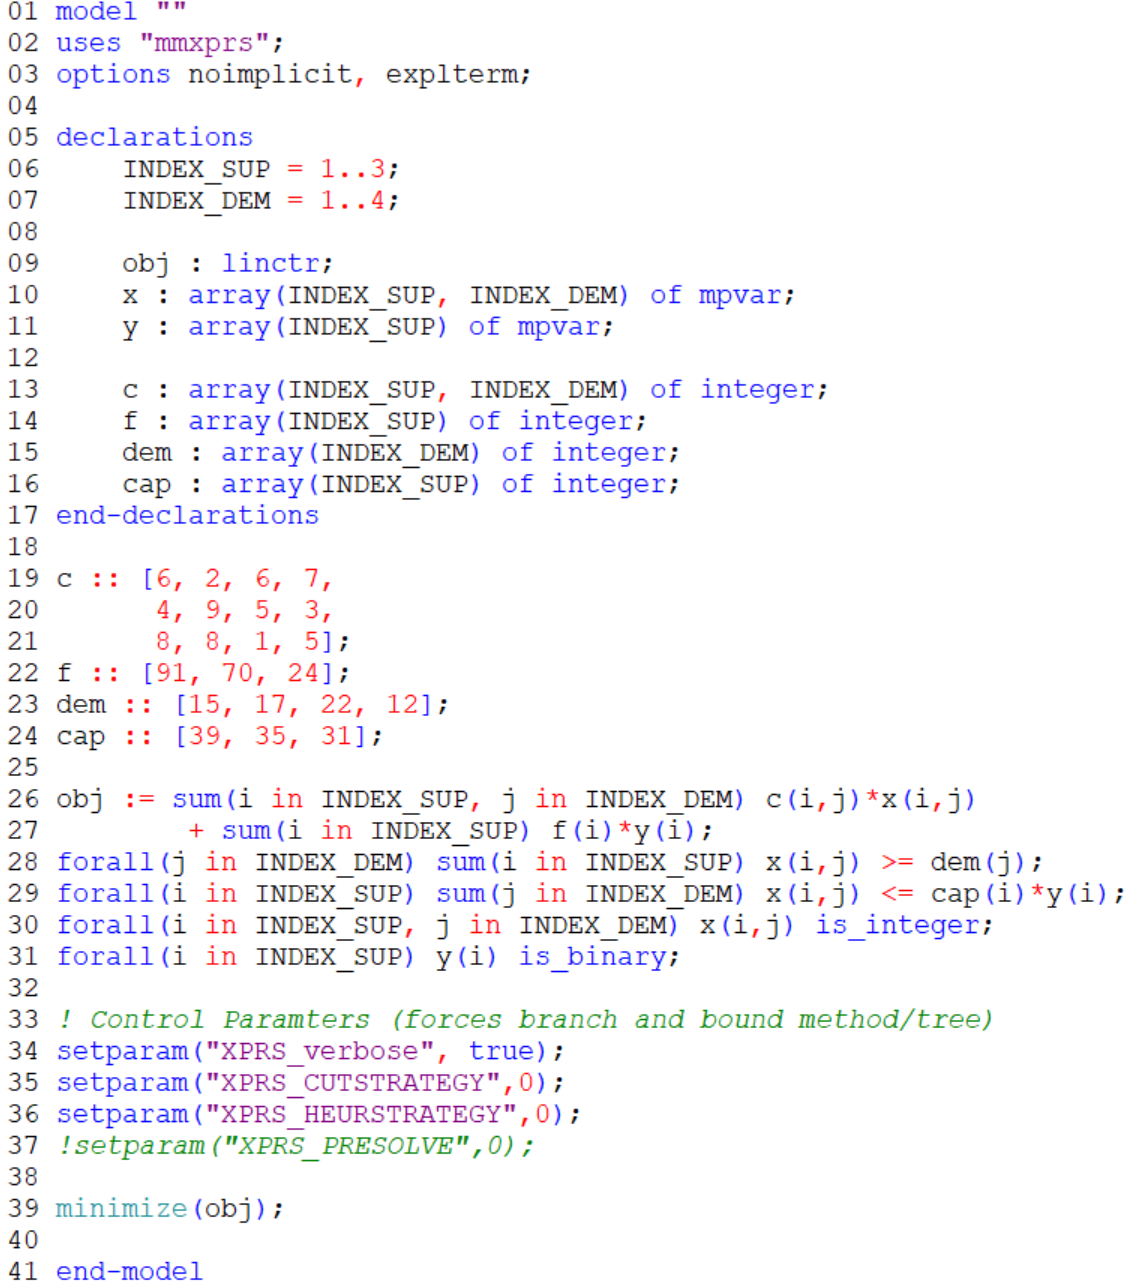
\includegraphics[width=\textwidth]{code2.png}
\end{center}

\newpage
\newpage
\begin{pbox}
    Report the solution and solver details. Discuss whether the solution makes sense for planning and management decision making.
\end{pbox}

Running the above code, Xpress produces the following integer/binary optimal solution using the branch and bound method (max depth 4), supported by the simplex dual algorithm.
\[
    Z = 327
    \qquad
    x = \mqty[
        15 & 17 & 0 & 3 \\
        0 & 0 & 0 & 0 \\
        0 & 0 & 22 & 9
    ]
    \qquad
    y = \mqty[1 \\ 0 \\ 1]
\]
This solution, in contrast to that of the unrestricted type implementation, can be properly interpreted in terms of the actual problem. The values of $y$ indicate that the first and third factories should be upgraded and kept open, while the second factory should be closed. The values of $x$ tell us how many units the factories should be supplying to each of the four customers, where $x_{ij} = n$ tells us that factory $i$ should supply $n$ units to customer $j$. Moreover, because of the correct binary form of the $y$ variables, the value of the objective function should accurately reflect the real costs associated to this solution (and manually computing the total cost for the given production numbers confirms that the objective value is indeed correct). Hence, we conclude that P\&G should expect to spend no less than $327$ (money units) in order to refurbish their soaps and detergents production lines, while continuing to meet their customers demands, and can expect to spend exactly that much by implementing the stated solution.

\end{document}